\documentclass[11pt,a4paper]{ctexart}

\usepackage{amsmath,amssymb,amsthm,mathtools}
\usepackage{booktabs,tabularx,multirow}
\usepackage{graphicx,float}
\usepackage{xcolor}
\usepackage{geometry}
\usepackage{hyperref}
\usepackage{listings}
\usepackage{enumitem}

\geometry{left=2.3cm,right=2.3cm,top=2.4cm,bottom=2.4cm}
\hypersetup{colorlinks=true,linkcolor=blue!60!black,citecolor=blue!60!black,urlcolor=blue!60!black}
\graphicspath{{../results/figures/}}
\setlength{\parindent}{2em}
\setlength{\parskip}{0.25em}
\newtheorem{theorem}{定理}[section]
\newtheorem{proposition}[theorem]{命题}
\theoremstyle{definition}
\newtheorem{definition}[theorem]{定义}
\newcommand{\E}{\mathbb{E}}
\newcommand{\ind}{\mathbb{I}}

\lstset{
  basicstyle=\ttfamily\small,
  backgroundcolor=\color{gray!8},
  frame=single,
  breaklines=true,
  columns=fullflexible
}

\title{机器学习数据获取与数据定价\\
\large 《Optimal Pricing for Data-Augmented AutoML Marketplaces》复现与改进阶段报告}
\author{课程大作业 C.3}
\date{2026年7月16日\quad 版本 0.1.0}

\begin{document}
\maketitle

\begin{abstract}
本文复现 Han 等人提出的数据增强型 AutoML 市场的核心机制：平台将买家数据与外部数据连接，联合搜索增强数据和模型，并按模型性能定价。理论部分实现了买家的马尔可夫最优停止动态规划、样本轨迹上的价格曲线优化以及基于停止时间的买家先验学习。我们进一步指出，论文的经验定价程序式 (7)/(8) 与正文的“自愿购买”叙述存在不一致：程序强制每个买家从已发现模型中选择一个，即使所有模型的净效用均为负。为此，我们加入不购买外部选项，得到满足个体理性（IR）的价格优化，并扩展为在多个候选买家先验上最大化最坏收入的鲁棒 IR 定价。固定随机种子的合成实验显示，论文式目标预测收入为 0.488，但真实允许退出后同分布测试收入仅为 0.275；IR 定价将其提高到 0.375（$+36.3\%$）。不利先验偏移下，鲁棒 IR 收入为 0.280，相比论文式价格提高 $153.6\%$，相比普通 IR 再提高 $15.1\%$。先验学习实验的 KL 散度由 0.0311 降至 0.0069。本文同时说明复现边界：当前结果验证的是机制与改进，而不是对原文 69K 数据集池实验的逐点重现。
\end{abstract}

\tableofcontents
\newpage

\section{问题描述与研究动机}

标准 AutoML 平台主要搜索模型和超参数，并按计算时间收费。论文~\cite{han2023}考虑另一类市场：买家只有少量训练数据，平台拥有可连接的外部数据池。平台一边寻找有用的增强特征，一边搜索模型，并持续向买家展示当前最优性能。买家可以决定继续搜索还是停止，并可购买已发现模型。

该问题把两个通常分开的主题连接起来：其一是\textbf{数据获取}，即从大量外部表中寻找与当前任务有关的增强；其二是\textbf{数据定价}，即不直接出售原始表，而是按照增强最终带来的模型性能定价。核心困难在于：性能搜索是随机、序贯且有成本的，买家的性能估值又是私有信息，平台必须同时预判买家的停止行为与购买行为。

本文阶段工作的目标如下：
\begin{enumerate}[label=(\arabic*)]
  \item 理解并实现论文的马尔可夫最优停止、经验价格曲线和先验学习；
  \item 复现论文 RQ2/RQ3 所研究的定价与学习现象；
  \item 找出机制中的可操作问题，给出理论修正并通过实验比较；
  \item 建立可重复运行、可测试、可生成 PDF、可版本化管理的项目工程。
\end{enumerate}

\section{论文整体思路与建模}

\subsection{市场参与者与性能过程}

令离散性能集合为 $\mathcal Q=\{q_1,\dots,q_K\}$，搜索时刻为 $t=1,\dots,T$。当前性能按照时变马尔可夫链演化：
\[
  P^t(q'\mid q)=\Pr(Q_{t+1}=q'\mid Q_t=q).
\]
买家私有类型为 $\theta\in\Theta$，类型决定估值曲线 $v^\theta(q)$；平台仅知道类型先验 $\mu(\theta)$。平台事先发布统一价格曲线 $x:\mathcal Q\to\mathbb R_+$。若买家在时刻 $\tau$ 停止并购买性能 $q$ 的模型，效用为
\[
  u^\theta(q,\tau)=v^\theta(q)-x(q)-c\tau,
\]
其中 $c$ 是每轮真实发现成本。平台的主要收入是模型支付 $x(q)$，发现成本 $c\tau$ 用于覆盖搜索成本。

\subsection{买家最优停止动态规划}

状态 $(q_1,q_2,t)$ 分别记录当前净价值最高的历史性能、当前性能和时刻。令 $\Phi(q_1,q_2,t)$ 为从该状态出发的最优期望效用，则论文的递推为
\begin{align}
\Phi(q_1,q_2,t)=\max\Big\{&v^\theta(q_1)-x(q_1)-ct,\\
&\E_{q\sim P^t(\cdot\mid q_2)}
\Phi\big(\arg\max_{r\in\{q_1,q\}}[v^\theta(r)-x(r)],q,t+1\big)\Big\}.
\end{align}

\begin{proposition}[论文 Proposition 4.1]
给定价格曲线、类型估值与转移矩阵，买家的最优停止策略可在 $O(|\mathcal Q|^2T)$ 时间内由动态规划计算。
\end{proposition}

\textbf{证明 insight。}未来性能仅依赖当前性能 $q_2$，历史只需保留“目前净价值最高的性能”$q_1$，因此状态空间是 $|\mathcal Q|^2T$。从 $T$ 时刻的强制停止边界条件向前递推，每个状态比较立即停止与继续一期的期望效用。若转移期望通过矩阵运算实现，总复杂度为论文给出的多项式量级；我们的实现保留了显式状态循环，便于逐项核对。

\subsection{样本轨迹上的价格曲线}

当发现成本相对估值可忽略时，论文把一条性能轨迹 $s=[q_1,\dots,q_T]$ 看成可购买质量集合，并定义
\[
q^*(\theta,x,s)\in\arg\max_{q\in s}\{v^\theta(q)-x(q)\}.
\]
经验收入目标为
\begin{equation}\label{eq:forced}
\max_x\sum_\theta\mu(\theta)\frac1m\sum_{s\in S}x(q^*(\theta,x,s)).
\end{equation}
论文使用二元变量 $z(\theta,s,q)$ 表示选择，连续变量 $y=x(q)z$ 表示支付，并用 Big-$M$ 约束将双层问题线性化为 MILP。

\begin{theorem}[论文 Theorem 4.2]
若发现成本可忽略、估值上界为 $b$，取
\[
m=\frac{b^2}{2\epsilon^2}\ln\frac{2}{\delta}
\]
条独立样本轨迹，则 MILP 得到的价格曲线以至少 $1-2\delta$ 的概率是总体最优价格曲线的加性 $\epsilon$ 近似。
\end{theorem}

\textbf{证明 insight。}第一步证明 MILP 精确表示有限样本上的最优响应和支付；第二步对固定价格曲线使用 Hoeffding 不等式控制经验收入与总体收入的偏差，再比较经验最优解与总体最优解。关键意义是：定价不要求显式恢复完整马尔可夫链，只需采样发现轨迹即可获得 PAC 风格保证。

\subsection{未知先验的贝叶斯学习}

论文根据观测到的停止轮次 $y^{(t)}$ 更新类型信念：
\[
w^{(t)}(\theta_i)=
\frac{\Pr(y^{(t)}\mid\theta_i,x^{(t)})\mu^{(t)}(\theta_i)}
{\sum_j\Pr(y^{(t)}\mid\theta_j,x^{(t)})\mu^{(t)}(\theta_j)},\qquad
\mu^{(t+1)}=(1-\eta_t)\mu^{(t)}+\eta_tw^{(t)}.
\]
在可识别性成立时，反复交互使估计先验趋近真实先验。论文进一步定义估计误差代价 CEE，即使用估计的 $(\mu,P)$ 定价而在真实 $(\mu^*,P^*)$ 下损失的收入。

\begin{theorem}[论文 Theorem 5.2]
若 $\|\mu-\mu^*\|_2\le\epsilon$ 且 $\|P-P^*\|_2\le\epsilon$，则估计错误导致的收入损失满足 $\mathrm{CEE}(\mu,P)=O(\epsilon)$。
\end{theorem}

证明思路是分别控制先验误差对收入加权的影响，以及转移矩阵扰动经动态规划递推产生的效用误差，再通过三角不等式合并。

\subsection{数据增强--模型发现}

暴力枚举增强集合和模型需要 $O(2^{|\mathcal P|}|\mathcal M|)$ 次训练。论文 Algorithm 2 在 Metam 数据发现框架上加入 Exp3 对抗多臂老虎机：每个模型视为一只臂，每轮只训练一个模型；增强候选通过相似性聚类及 Thompson/贪心策略选择。这一部分支撑原文 RQ1。由于论文使用的 69K NYC 数据集池及完整市场实现未公开，本阶段没有把较小的替代实验宣称为 Figure 3 的逐点复现。

\section{实现设计与可复现性}

代码分为四个核心模块：
\begin{itemize}
  \item \texttt{market.py}：马尔可夫轨迹采样、三维停止 DP、策略执行；
  \item \texttt{pricing.py}：式~\eqref{eq:forced}、IR 收入、价格候选网格与 independent baseline；
  \item \texttt{learning.py}：停止时间似然下的平滑贝叶斯更新；
  \item \texttt{experiments.py}：固定种子数据生成、训练/测试/OOS 评估和作图。
\end{itemize}

实验使用 $|\mathcal Q|=4$、$|\Theta|=6$、$T=6$、240 条训练轨迹和 4000 条测试轨迹。价格候选取每个质量上的 0 与所有类型估值，共精确枚举 $7^4=2401$ 条曲线。随机种子为 20260716。以下命令会依次运行测试、实验并编译本报告：
\begin{lstlisting}
make all
\end{lstlisting}
原始数值同时保存为 \texttt{results/summary.json} 与
\texttt{results/tables/pricing\_results.csv}，避免只能从图中读取结果。

\section{机制问题与改进方案}

\subsection{问题：定价程序缺少“不购买”选项}

正文称模型价格 $x(q)$ 是买家自愿支付，但式~\eqref{eq:forced} 以及 MILP 约束
$\sum_{q\in s}z(\theta,s,q)=1$ 强制每个类型在每条轨迹上选择一个模型。若
\[
\max_{q\in s}\{v^\theta(q)-x(q)\}<0,
\]
真实理性买家应不购买，而原程序仍选择“亏损最少”的模型并把 $x(q)$ 记为平台收入。因此，经验目标可能偏好不可实施的高价。

\subsection{改进一：个体理性（IR）外部选项}

加入虚拟选项 $\bot$，令 $v^\theta(\bot)=x(\bot)=0$，将选择集合改为
$s\cup\{\bot\}$：
\begin{equation}\label{eq:ir}
q^*_{\mathrm{IR}}\in\arg\max_{q\in s\cup\{\bot\}}
\{v^\theta(q)-x(q)\}.
\end{equation}
在 MILP 中只需增加 $z(\theta,s,\bot)$，保留选择和为 1，并固定其价格、估值和支付为 0；或者增加约束使购买选项的效用非负。

\begin{proposition}[IR 修正的性质]
式~\eqref{eq:ir} 对每个类型和轨迹均满足事后个体理性。对任意固定价格曲线，允许退出后的可实现收入不高于强制选择目标；两者相等当且仅当强制目标选择的模型在所有正概率类型--轨迹对上均具有非负净效用（忽略零效用处的平局规则）。
\end{proposition}

\textbf{证明。}外部选项效用为 0，因此最优选择的效用至少为 0，得到个体理性。强制选择与 IR 选择的差异只发生在所有模型效用均小于 0 的事件上；强制目标在该事件中记录正价格，IR 目标记录 0，故前者逐样本不小于后者。没有此类正概率事件时两目标一致，反之严格产生虚假支付。\hfill$\square$

\subsection{改进二：先验偏移下的鲁棒 IR 定价}

真实市场的类型先验会变化。设 $\mathcal U$ 是由当前估计先验、均匀先验、低支付意愿偏移和高支付意愿偏移组成的候选集合，我们求解
\[
\max_{x\ge0}\min_{\mu\in\mathcal U}
\E_{\theta\sim\mu,s\sim S}[x(q^*_{\mathrm{IR}}(\theta,x,s))].
\]
该 max--min 目标牺牲部分同分布平均收入，换取先验变化时的收入下界。小规模实验仍可精确枚举；大规模版本可在原 MILP 上增加场景收入变量 $r$，并对每个 $\mu\in\mathcal U$ 加入 $r\le\mathrm{Rev}_{\mu}(x)$。

\section{实验结果与分析}

\subsection{定价结果}

\begin{table}[H]
\centering
\caption{价格机制收入比较。所有“实现收入”均允许买家不购买。}
\begin{tabular}{lrrrr}
\toprule
机制 & 论文式训练目标 & 训练实现 & IS 测试 & OOS 测试\\
\midrule
Paper forced-choice & 0.4881 & 0.2687 & 0.2749 & 0.1106\\
Independent & 0.3361 & 0.3245 & 0.3280 & 0.2169\\
IR-aware（本文） & 0.4161 & \textbf{0.3661} & \textbf{0.3746} & 0.2436\\
Robust IR（本文） & 0.3426 & 0.3327 & 0.3367 & \textbf{0.2805}\\
\bottomrule
\end{tabular}
\label{tab:pricing}
\end{table}

\begin{figure}[H]
\centering
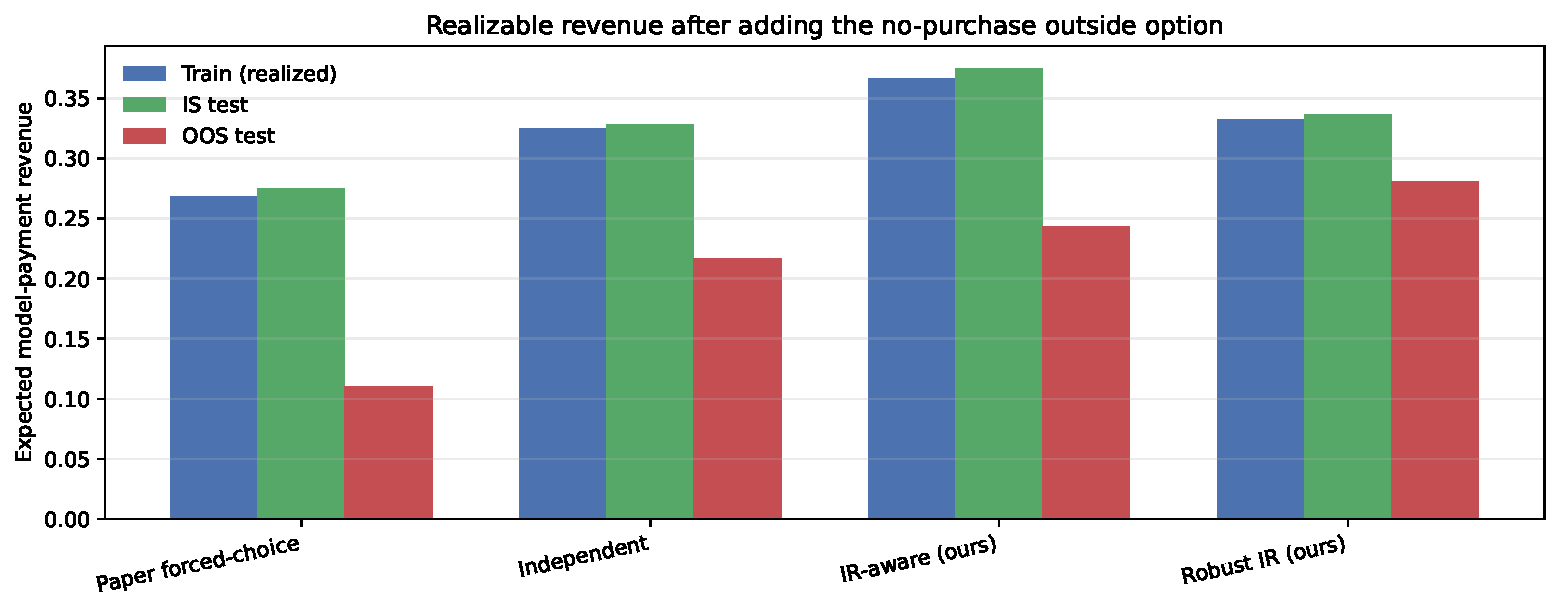
\includegraphics[width=0.94\textwidth]{pricing_comparison.pdf}
\caption{加入不购买选项后，各价格曲线的可实现收入。OOS 将更多概率质量移向低支付意愿类型。}
\label{fig:pricing}
\end{figure}

论文式强制选择解的训练目标为 0.4881，但训练实现收入只有 0.2687，说明目标中包含大量不会发生的支付。其价格曲线为 $(0.22,0.39,0.70,1.02)$；按类型先验计，80\% 的类型在至少一类可达集合上会因负效用而退出。IR-aware 直接优化真实购买行为，在 IS 测试上达到 0.3746，相比论文式价格提高 36.3\%。

OOS 场景把先验更多地移向低支付意愿类型。普通 IR 收入从 0.3746 降为 0.2436，而鲁棒 IR 采用更平缓的价格 $(0.20,0.25,0.31,0.50)$，获得 0.2805：相对普通 IR 提高 15.1\%，相对论文式价格提高 153.6\%。代价是 IS 收入比普通 IR 低 10.1\%。这符合 max--min 定价的预期权衡。

\subsection{先验学习结果}

为满足论文的可识别性要求，我们设置一个零模型价格的短期探索阶段，并保留每轮发现成本 $c=0.03$。不同估值曲线因“继续等待高性能”的意愿不同而产生不同停止时间分布。每轮使用 100 个买家观测，学习率为 $1/\sqrt t$。

\begin{figure}[H]
\centering
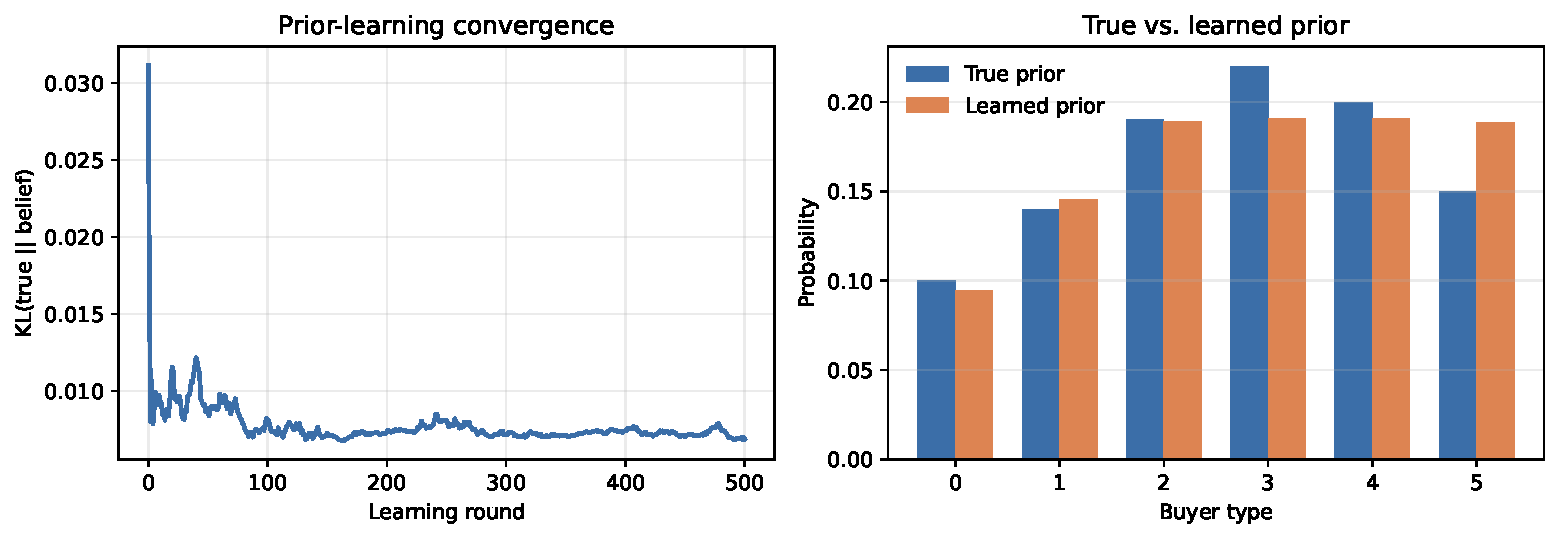
\includegraphics[width=0.94\textwidth]{prior_learning.pdf}
\caption{基于停止轮次的买家类型先验学习。}
\label{fig:learning}
\end{figure}

KL 散度从均匀初始化时的 0.0311 降至 0.0069，复现了论文 RQ3 的定性结论：只观察停止时间也能逐步恢复类型先验。但类型 4--6 的停止分布仍较接近，最终概率存在混淆；这也说明论文定理中的“可识别性”不是自动成立的，平台需要设计具有信息量的探索价格或收集额外行为信号。

\subsection{运行结果与测试证据}

\begin{lstlisting}
$ make test
Ran 4 tests in 0.025s
OK

$ make experiment
Completed 4 pricing schemes.
Results: results/summary.json
\end{lstlisting}

单元测试覆盖：马尔可夫采样可重复性、DP 的继续/停止判断、缺少外部选项产生不可实现收入，以及单质量情形下 IR 网格解与垄断价格的一致性。

\section{局限性、后续计划与中期展示安排}

当前阶段完成了机制级复现，但尚有三项重要边界。第一，论文的大规模 NYC 数据池和作者完整实现未公开，因此尚未复现 Data-Bandit 的 Figure 3；第二，当前精确网格只适用于小 $|\mathcal Q|$，最终版本应增加 Gurobi/SCIP 的 MILP 接口；第三，当前主要表格是单随机种子结果，最终报告需增加多种子置信区间。

后续按以下顺序推进：
\begin{enumerate}[label=(\arabic*)]
  \item 在公开表格任务上实现简化的 augmentation--model Exp3，完成 RQ1；
  \item 在 $|\mathcal Q|=20,|\Theta|=20,m=100$ 的论文设置上运行 MILP；
  \item 对先验偏移强度、发现成本和转移矩阵估计误差做消融实验；
  \item 运行 20--50 个随机种子并报告均值、标准差和显著性；
  \item 制作中期展示：理论 4 页、实现与复现 3 页、问题和改进 3 页、计划 1 页；
  \item 将本报告扩写为最终报告，补齐 RQ1 截图、完整实验环境与附录证明。
\end{enumerate}

\section{结论}

本文建立了一个可运行、可测试和可版本化的复现工程，实现了论文的最优停止、经验定价与先验学习核心。机制分析发现，论文经验程序缺少“不购买”选项，会把负效用买家的强制支付误记为收入。加入外部选项后，定价目标与正文的自愿购买语义一致，并在合成实验中显著提高可实现收入。进一步的鲁棒 IR 定价对买家先验偏移表现更稳定。当前证据支持该改进的理论正确性和实验有效性，但最终结论仍需通过多种子、大规模 MILP 和真实表格数据实验加强。

\begin{thebibliography}{9}
\bibitem{han2023}
Y. Han, S. Padmanabha, S. Wang, Z. Huang, and J. Zhao.
\newblock Optimal Pricing for Data-Augmented AutoML Marketplaces.
\newblock arXiv preprint, 2023 (local manuscript revision used in this project).
\end{thebibliography}

\end{document}

